\documentclass[10pt]{article}

% Language setting
% Replace `english' with e.g. `spanish' to change the document language
\usepackage[english]{babel}

% Set page size and margins
% Replace `letterpaper' with`a4paper' for UK/EU standard size
\usepackage[a4paper,top=2cm,bottom=2cm,left=3cm,right=3cm,marginparwidth=1.75cm]{geometry}

% Useful packages
\usepackage{amsmath}
\usepackage{tikz}
\usepackage{graphicx}
\usepackage{mwe}
\usepackage{fullpage}
\usepackage{hyperref}
\hypersetup{linkcolor=blue, urlcolor=blue, colorlinks}
\usepackage{caption}
\usepackage{subcaption}
\usepackage{float}
\usepackage{enumerate}

\title{Assignment 4: Kokkos \\ \large \textit{Accelerator-based Programming}}
\author{Oskar Tegby}
\date{October 2022}

\setlength{\parindent}{0pt}

\begin{document}
\maketitle

\begin{tikzpicture}[remember picture, overlay]
  \node [anchor=north west, inner sep=25pt]  at (current page.north west)
     {
\includegraphics[height=3.3cm]{uppsala-universitet-logo.png}};
\end{tikzpicture}

\section{Introduction}
This assignment studies the computational bandwidths that a computational kernel have on the GPU when implemented using Kokkos. The bandwidth is tested using finite element matrices arising from a 3D discretization of the Laplacian on a mesh of simplices. Notably, the computations using these matrices are completely parallelizable. In this report, we discuss the performance that we achieve using various settings in Kokkos. All tests were run on the Snowy node of the UPPMAX cluster.
\section{Tasks}
\subsection{Task 1 and 2}
In Figure \ref{fig:best_both_melems}, we observe the measure million elements computed per seconds (MELEM/s) computed using the layout which is appropriate for the corresponding device. That is, for CPUs we want \texttt{LayoutRight} (row-major) to get contigous memory loads, and for GPUs we want \texttt{LayoutLeft} (column-major) in order to coalesce the memory accesses. \\

Given that application is fully parallelizable and lacks divergent computations, the computations on the GPU should be performed much faster than on the CPU, which has much fewer ALUs running in parallel. However, somewhat surprisingly, the GPU performs better than the CPU by a factor 10 in our measurements. This observation strongly suggests that the memory bandwidth is limiting the performance. \\

In order to examine the veracity of that belief, we study Figure \ref{fig:best_both_gbps} and Figure \ref{fig:best_both_gflops}. There, we observe that the peak throughput is about 210 GB/s for the GPU, and 50 GB/s for the CPU. However, here, it is crucial to recall that the ratio between the data transfer and the compute dictates the performance on the graphics card. That is, we may have a higher throughput on the GPU than the CPU, but if we only perform a few floating-point operations on each data, then that will not matter.
\begin{figure}[!ht]
    \centering
    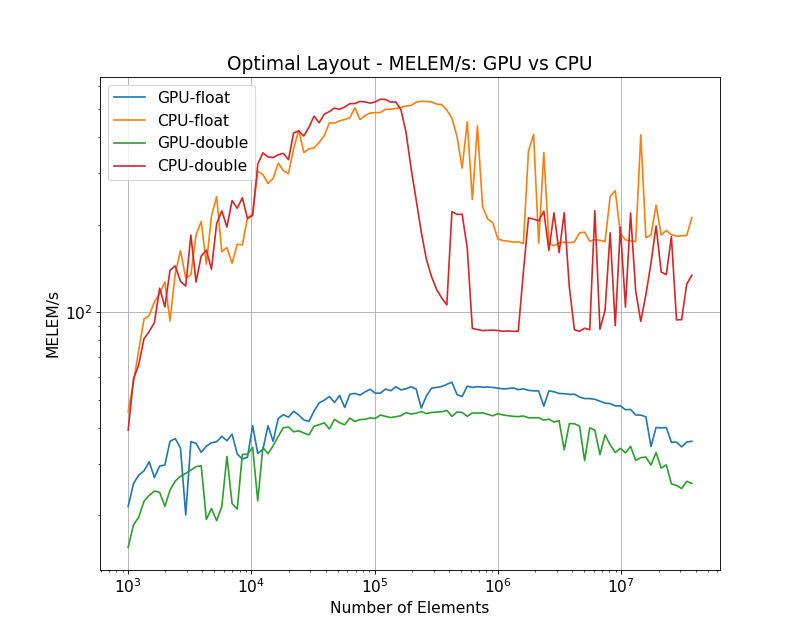
\includegraphics[width=0.49\textwidth]{figs/best_both_melems.png}
    \caption{Optimal layouts on the CPU and GPU, respectively, using \texttt{single} and \texttt{double} precision.}
    \label{fig:best_both_melems}
\end{figure}
\begin{figure}[!ht]
    \centering
    \begin{subfigure}[b]{0.49\textwidth}
        \centering
        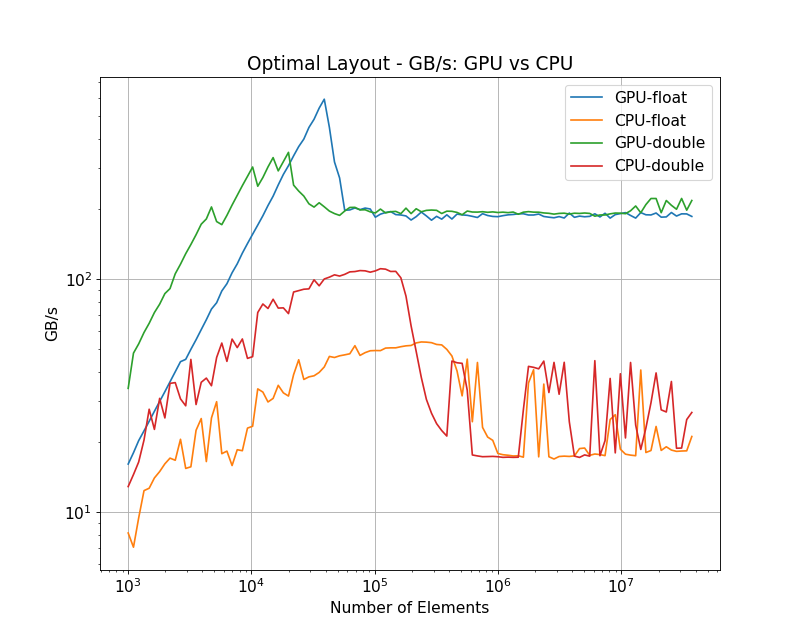
\includegraphics[width=\linewidth]{figs/best_both_gbps.png}
        \caption{The throughput of the computation.}
        \label{fig:best_both_gbps}
    \end{subfigure}\hfill
    \begin{subfigure}[b]{0.49\textwidth}
        \centering
        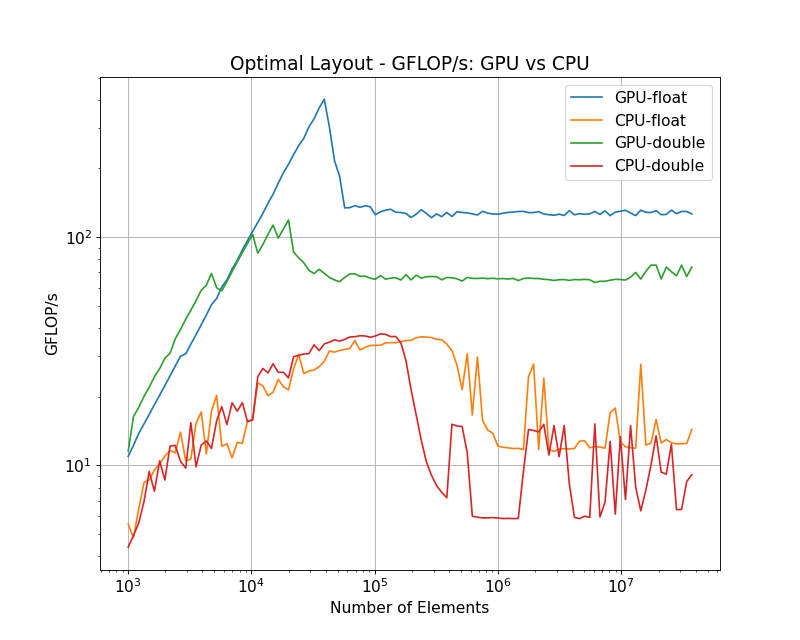
\includegraphics[width=\linewidth]{figs/best_both_gflops.png}
        \caption{The FLOPS of the computation.}
        \label{fig:best_both_gflops}
    \end{subfigure}\hfill
    \caption{The throughput and FLOP/s achieved during the computations.}
    \label{fig:best_gbps_and_flops}
\end{figure}
\subsection{Task 3}
The theoretical throughput of this GPU is 320 GB/s, and we are loading 9 floats for the J matrix since it is $3\times3$ and 16 floats for the A matrix since it is $4\times4$. Thus, we are loading 25 floats, each of which are 4 bytes, for every of the $N$ matrices. \\

Thus, we load the data from the CPU's RAM to the RAM of the GPU in
\begin{align*}
    \frac{N\cdot25\cdot4}{260}=2.56N
\end{align*}
nanoseconds over the PCIe interface. Furthermore, the computations on the GPU take
\begin{align*}
    \frac{N\cdot68}{8}\approx 12N
\end{align*}
picoseconds since the computational power of the GPU is 8 TFLOP/s and we are performing 68 FLOP per iteration. Clearly, the limit lies in the interconnect since it is a factor of a thousand higher than that of the computation time.
\subsection{Task 4}
In order to study the differences in data layouts, we study Figure \ref{fig:all_melems_gpu} and Figure \ref{fig:all_melems_cpu}. The theory tells us that \texttt{LayoutLeft} should be better for the GPU since it naturally coalesces the memory accesses, and that \texttt{LayoutRight} should be better for the CPU since it instead gives contiguous memory accesses. \\

Again, surprisingly, we observe in Figure \ref{fig:all_melems_gpu} that the opposite results are observed for the GPU compared to our expectations. A possible answer could be that the memory accesses somehow are misaligned because of the misaligning memory accesses when the CPU is sending the data to the GPU. However, that is not what is supposed to happen, so we are left unable to explain this behavior. \\

In Figure \ref{fig:all_melems_cpu}, we instead observe the expected behavior, that \texttt{LayoutRight} indeed results in a higher throughput. In both cases, we, of course, observe that floating-point precision trumps double-point precision since we divide the size of the data being sent in half. We also observe that ratio somewhat in Figure \ref{fig:all_melems_gpu} where the memory hierarchy is less pronunced, but less so in Figure \ref{fig:all_melems_cpu}. There, we instead observe that the spikes resulting from cache accesses occur at different problem sizes instead. That is, the graphs are clearly shifted rightwards instead of upwards for the CPU.
\begin{figure}[!ht]
    \centering
    \begin{subfigure}[b]{0.49\textwidth}
        \centering
        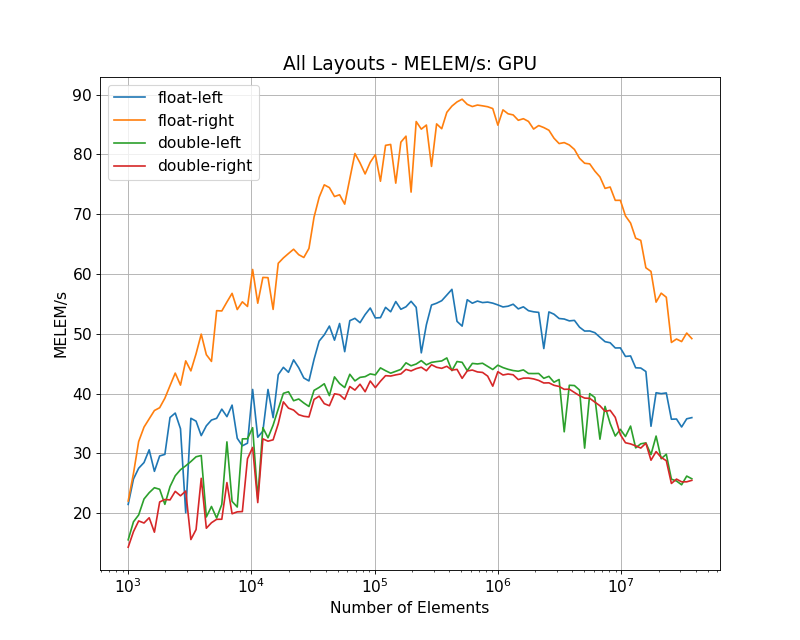
\includegraphics[width=\linewidth]{figs/all_melems_gpu.png}
        \caption{The GPU with LayoutLeft and LayoutRight.}
        \label{fig:all_melems_gpu}
    \end{subfigure}\hfill
    \begin{subfigure}[b]{0.49\textwidth}
        \centering
        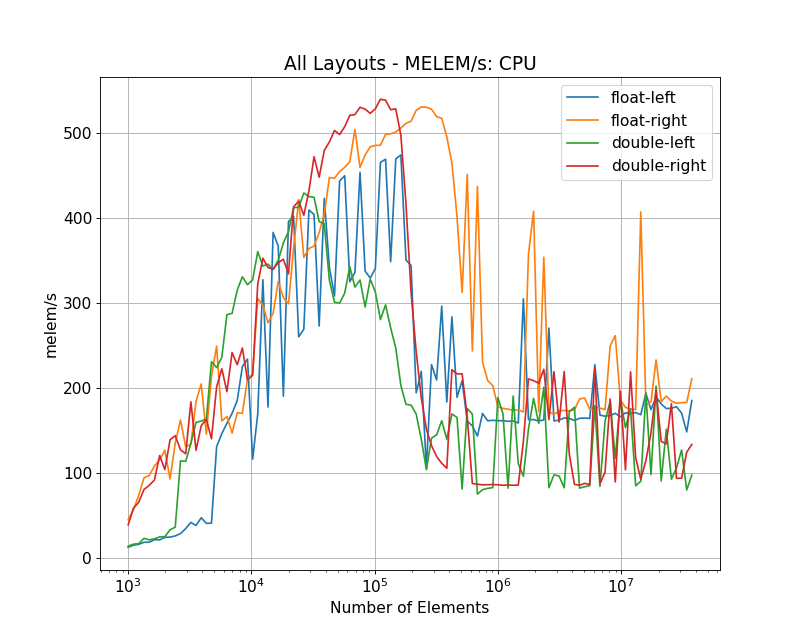
\includegraphics[width=\linewidth]{figs/all_melems_cpu.png}
        \caption{The CPU with LayoutLeft and LayoutRight.}
        \label{fig:all_melems_cpu}
    \end{subfigure}\hfill
    \caption{The MELEM/s on the GPU and CPU with \texttt{single} and \texttt{double} precision, respectively.}
    \label{fig:all_melems}
\end{figure}
\subsection{Task 5}
In order to study the ratio between the compute and the transfer, we plot the transfer time between the CPU and the GPU, and the execution time of the kernel itself when the data is on the GPU. We find these results in Figure \ref{fig:all_copykernel_gpu}. There, we observe that the transfers back and forth dominate the execution time. \\

Here, using the notation \textbf{l} for \texttt{LayoutLeft} and \textbf{r} for \texttt{LayoutRight}, as well as \textbf{f} for \texttt{float} and \textbf{d} for \texttt{double}, we observe that the transfer of floating-point precision data with \texttt{LayoutLeft} is the fastest one, and that double precision with \texttt{LayoutRight} is among the slower ones. That is to be expected as we now have discussed at length.

\begin{figure}[!ht]
    \centering
    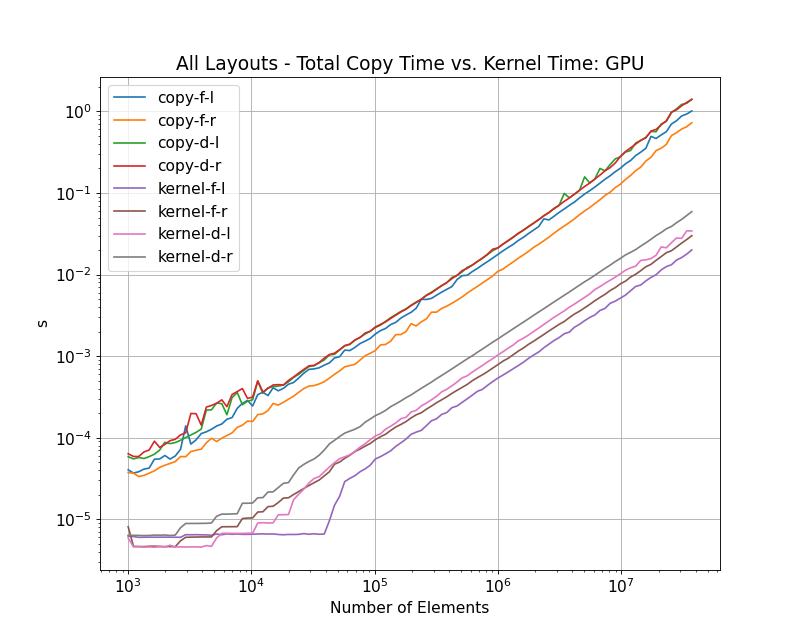
\includegraphics[width=0.49\textwidth]{figs/all_copykernel_gpu.png}
    \caption{The time it takes to transfer the data and execute the kernel, respectively.}
    \label{fig:all_copykernel_gpu}
\end{figure}

Notably, the former contradicts the earlier results showing that the usage of floating-point data gave a lower throughput, which supports the notion that there is some other factor at play in that scenario. 
\subsection{Task 6}
The issue here clearly lies in the ratio between memory transfer and the amount of computations performed on the data being sent back and forth. This means that we should not off-load computations to the GPU unless there is a significant amount of computations being done on each element. \\

Here, this motivates keeping the computation of the Jacobians on the CPU since it would be absurd to sense so little data to compute them on the GPU. The reason is that we would not need the vertices and connectivity information after we have computed the Jacobians, so sending it that data will be useless for the rest of the computation. Furthermore, the vertices are likely to affect more than one value in the Jacobian, so that having a more advanced pipeline which better handles divergent computation and unorderely data movement yields a greater impact on performance. However, that will be insignificant here when compared to the transfer time of the data itself. \\

As observed in Figure \ref{fig:best_both_melems}, the CPU beat the GPU in this setting, so it is unreasonable that this part of the pipeline should be off-loaded to the GPU. However, when computing sparse matrices, we do not need to send nearly as much data due to the sparsity. Thus, it is plausible that they will be computed much faster on the GPU if they are large enough, given the usage of data structures for sparse matrices. \\

Lastly, solving a linear system with an iterative solver is a typical application for the GPU since we need to perform many operations on the same data, often containing several parallel steps such as in conjugate gradient (as used in FGMRES). Thus, it should be off-loaded on the GPU if enough iterations are needed to solve the linear system of equations.
\end{document}
